\chapter{Literature Review}
\label{chap:literature}

% Outline approved 2 November 2026 (notes/chapter2-outline.md). Sources for
% every claim are listed in notes/chapter2-claims.md.

\section{Introduction}
\label{sec:lit-intro}

This chapter reviews the background on which the study rests and the work closest to it. It first describes the Long Term Evolution (LTE) downlink signal that the detectors must find (\cref{sec:lte}) and places occupancy detection within cognitive radio and dynamic spectrum access (\cref{sec:cr}). It then reviews classical spectrum sensing, giving most space to energy detection, the baseline against which the autoencoder is judged (\cref{sec:sensing}). The receiver is described in \cref{sec:sdr} and the time--frequency representation used as model input in \cref{sec:stft}. \Cref{sec:ae} introduces autoencoders and their use for anomaly detection, including the choice between fully connected and convolutional architectures. Related work is reviewed by theme in \cref{sec:related}, the research gap is stated in \cref{sec:gap}, and \cref{sec:lit-summary} summarizes the chapter.

\section{The LTE Downlink}
\label{sec:lte}

An occupancy detector for LTE needs a clear picture of what an active LTE carrier transmits. This section summarizes the parts of the LTE physical layer that matter for detection: how the downlink signal is organized in time and frequency, which channel bandwidths and operating bands are defined, and which signals a carrier transmits at all times. The sources are the technical specifications of the 3rd Generation Partnership Project (3GPP), in the versions published by the European Telecommunications Standards Institute \parencite{3gpp2026a,3gpp2026b}.

\subsection{OFDM Resources and Frame Structure}
\label{sec:lte-frame}

The LTE downlink transmits orthogonal frequency-division multiplexing (OFDM) symbols \parencite[clause~6.12]{3gpp2026a}. Its resources form a grid of subcarriers in frequency and OFDM symbols in time. With the normal cyclic prefix and a subcarrier spacing of \qty{15}{\kilo\hertz}, a resource block spans 12 subcarriers, or \qty{180}{\kilo\hertz}, and seven OFDM symbols, which make up one slot \parencite[Table~6.2.3-1]{3gpp2026a}. In frequency-division duplex (FDD) operation, uplink and downlink are separated in frequency. FDD uses frame structure type~1, in which a radio frame lasts \qty{10}{\milli\second} and consists of ten subframes of \qty{1}{\milli\second}, numbered 0 to 9; each subframe consists of two slots of \qty{0.5}{\milli\second} \parencite[clause~4.1]{3gpp2026a}. A frame therefore contains 20 slots, numbered 0 to 19. \Cref{fig:lte-frame} shows this hierarchy together with the positions of the synchronization signals described in \cref{sec:lte-sync}. Only FDD bands are considered in this study (\cref{sec:lte-bands}).

\begin{figure}[tbp]
  \centering
  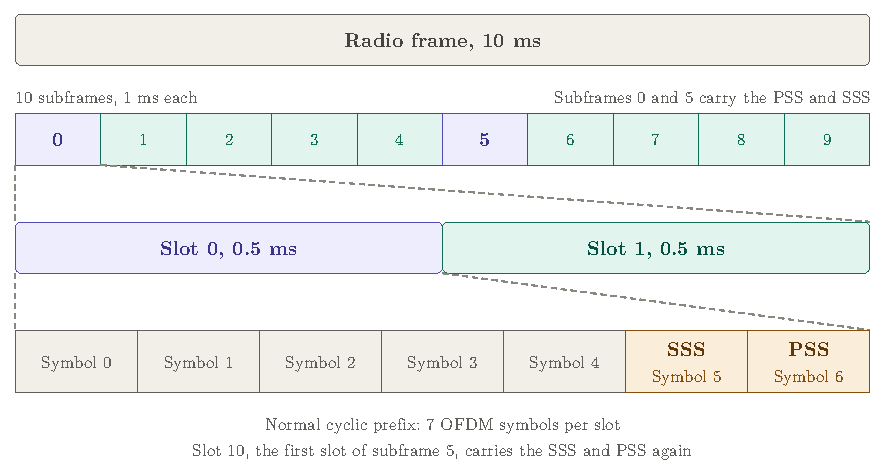
\includegraphics[width=\textwidth]{fig2-lte-frame-sync}
  \caption[Frame structure of the LTE FDD downlink]{Frame structure of the LTE FDD downlink (frame structure type~1) with the normal cyclic prefix. Subframes 0 and 5 carry the secondary and primary synchronization signals (SSS and PSS) in the last two OFDM symbols of their first slot. Drawn from the definitions in \textcite[clauses~4.1, 6.11.1.2 and 6.11.2.2; Table~6.2.3-1]{3gpp2026a}.}
  \label{fig:lte-frame}
\end{figure}

\subsection{Channel Bandwidths and Operating Bands}
\label{sec:lte-bands}

An LTE carrier has one of six channel bandwidths, from \qty{1.4}{\mega\hertz} to \qty{20}{\mega\hertz}, each with a fixed number of resource blocks, its transmission bandwidth configuration \parencite[Table~5.6-1]{3gpp2026b}. Because a resource block is \qty{180}{\kilo\hertz} wide, the resource blocks of a carrier occupy slightly less than its nominal channel bandwidth (\cref{tab:lte-bandwidths}). The receiver used in this study observes at most about \qty{2.56}{\mega\hertz} at a time \parencite{rtlsdrblog2024}. Only the smallest channel bandwidth, \qty{1.4}{\mega\hertz}, fits entirely within that window; of every larger carrier, only a slice is observed.

\begin{table}[tbp]
  \centering
  \caption[LTE channel bandwidths and resource blocks]{LTE channel bandwidths, their transmission bandwidth configurations, and the width occupied by the resource blocks. Sources: \textcite[Table~5.6-1]{3gpp2026b}; resource-block width from \textcite[Table~6.2.3-1]{3gpp2026a}; window width from \textcite{rtlsdrblog2024}.}
  \label{tab:lte-bandwidths}
  \begin{tabular}{S[table-format=2.1] S[table-format=3.0] S[table-format=2.2] c}
    \toprule
    {Channel} & {Resource} & {Occupied} & {Within a \qty{2.56}{\mega\hertz}} \\
    {bandwidth (\unit{\mega\hertz})} & {blocks} & {width (\unit{\mega\hertz})} & {window?} \\
    \midrule
     1.4 &   6 &  1.08 & Yes \\
     3   &  15 &  2.70 & No  \\
     5   &  25 &  4.50 & No  \\
    10   &  50 &  9.00 & No  \\
    15   &  75 & 13.50 & No  \\
    20   & 100 & 18.00 & No  \\
    \bottomrule
  \end{tabular}
\end{table}

The same specification defines the operating bands, with paired uplink and downlink ranges for FDD \parencite[Table~5.5-1]{3gpp2026b}. \Cref{tab:lte-bands} lists the downlink ranges of six FDD bands and shows whether each lies within the tuning range of the receiver, which extends to \qty{1.766}{\giga\hertz} \parencite{rtlsdrblog2024}. Bands~5, 8, 20 and~28 can be received; Bands~3 and~7 cannot. The band studied in this thesis is chosen in Chapter~3.

\begin{table}[tbp]
  \centering
  \caption[Downlink ranges of six LTE FDD bands]{Downlink ranges of six LTE FDD operating bands and whether each lies within the tuning range of the RTL-SDR Blog V4 (\qtyrange{0.5}{1766}{\mega\hertz}). Sources: \textcite[Table~5.5-1]{3gpp2026b}; \textcite{rtlsdrblog2024}.}
  \label{tab:lte-bands}
  \begin{tabular}{l c c}
    \toprule
    Band & Downlink range (\unit{\mega\hertz}) & Within the receiver's range? \\
    \midrule
    28 & \numrange{758}{803}   & Yes \\
    20 & \numrange{791}{821}   & Yes \\
    5  & \numrange{869}{894}   & Yes \\
    8  & \numrange{925}{960}   & Yes \\
    3  & \numrange{1805}{1880} & No  \\
    7  & \numrange{2620}{2690} & No  \\
    \bottomrule
  \end{tabular}
\end{table}

\subsection{Synchronization and Reference Signals}
\label{sec:lte-sync}

Every LTE cell transmits two synchronization signals, which a terminal uses to find the cell and its timing. There are 504 physical-layer cell identities, grouped into 168 cell-identity groups of three identities each; the primary synchronization signal (PSS) is generated from the identity within the group and the secondary synchronization signal (SSS) from the group \parencite[clauses~6.11, 6.11.1.1 and 6.11.2.1]{3gpp2026a}. The PSS is a frequency-domain Zadoff--Chu sequence of length~62. In FDD it is mapped to the last OFDM symbol of slots 0 and~10, that is, once every \qty{5}{\milli\second} \parencite[clauses~6.11.1.1 and 6.11.1.2]{3gpp2026a}. The SSS, an interleaved concatenation of two binary sequences of length~31, occupies the symbol before the PSS in the same slots \parencite[clauses~6.11.2.1 and 6.11.2.2]{3gpp2026a}. Both signals are mapped to the 62 subcarriers around the centre of the carrier, and the five subcarriers on each side are reserved and left empty. The two signals therefore occupy the central 72 subcarriers, six resource blocks or \qty{1.08}{\mega\hertz}, whatever the channel bandwidth \parencite[clauses~6.11.1.2 and 6.11.2.2]{3gpp2026a}.

A cell also transmits cell-specific reference signals (CRS). A terminal may assume that they are transmitted in all downlink subframes of an FDD cell that supports downlink data transmission \parencite[clause~6.10.1]{3gpp2026a}. In subframes configured for multicast and broadcast transmission (MBSFN subframes), they are transmitted only in the first one or two OFDM symbols \parencite[clauses~6.1 and 6.10.1.2]{3gpp2026a}.

Two consequences follow for this study. First, an active LTE carrier is never silent: even with no user traffic, its reference signals are transmitted in every downlink subframe and its synchronization signals every \qty{5}{\milli\second}. Occupancy in this thesis therefore means the presence of a carrier in the observed slice, not the traffic it carries, and idle reference data cannot be taken from quiet periods of an active carrier (Chapter~3). Second, the synchronization signals are confined to the central \qty{1.08}{\mega\hertz} of a carrier, while the receiver observes at most about \qty{2.56}{\mega\hertz}, less than the occupied width of any carrier of \qty{3}{\mega\hertz} or more (\cref{tab:lte-bandwidths}). A window centred on a carrier contains both synchronization signals, but a window placed elsewhere on the carrier contains neither (\cref{fig:obs-window}). A detector that relies on the synchronization signals, such as the correlator reviewed in \cref{sec:waveform}, can therefore work only when the window covers the centre of the carrier. Detectors based on energy, or on the spectrogram as a whole, can respond to any part of it.

\begin{figure}[tbp]
  \centering
  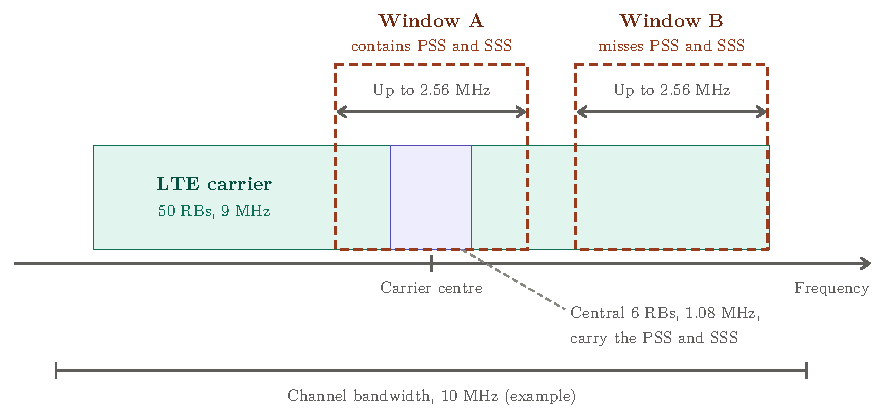
\includegraphics[width=\textwidth]{fig2-observation-window}
  \caption[Receiver window and an LTE carrier]{An example \qty{10}{\mega\hertz} LTE carrier (50 resource blocks, \qty{9}{\mega\hertz} occupied) and two receiver windows of up to \qty{2.56}{\mega\hertz}, drawn to scale in frequency. Window~A, centred on the carrier, contains the PSS and SSS, which occupy the central six resource blocks; window~B, placed off-centre, contains neither. Based on \textcite[Table~5.6-1]{3gpp2026b}, \textcite[Table~6.2.3-1 and clause~6.11]{3gpp2026a} and \textcite{rtlsdrblog2024}.}
  \label{fig:obs-window}
\end{figure}

\section{Cognitive Radio and Dynamic Spectrum Access}
\label{sec:cr}

The term \emph{cognitive radio} was coined by Joseph Mitola \parencite[p.~203]{haykin2005}. \Textcite{mitola1999} described cognitive radio as an extension of software radio with model-based reasoning about radio etiquette, the set of radio frequency bands, air interfaces, protocols, and spatial and temporal patterns that moderate the use of the spectrum (p.~13). They regarded software radio as an ideal platform for cognitive radio (p.~13). The radio's behaviour was organized as a cognition cycle in which it observes its environment, orients itself, plans, decides and acts, with some forms of supervised and unsupervised learning (p.~18).

\Textcite{haykin2005} defined cognitive radio as an intelligent wireless communication system, built on a software-defined radio (SDR), that is aware of its environment, learns from it and adapts to statistical variations in the incoming radio frequency stimuli. It has two objectives: highly reliable communication whenever and wherever needed, and efficient use of the radio spectrum (p.~201). Haykin motivated the concept with measurements showing that some frequency bands are largely unoccupied most of the time, others are partially occupied, and the rest are heavily used (p.~201). This underutilization leads to the notion of a spectrum hole, which he defined as \enquote{a band of frequencies assigned to a primary user, but, at a particular time and specific geographic location, the band is not being utilized by that user} \parencite[p.~201]{haykin2005}. Spectrum utilization could be improved by allowing a secondary user, one not being served in the band, to access a spectrum hole at the right location and time (p.~201). \Cref{fig:spectrum-holes} illustrates the idea.

\begin{figure}[tbp]
  \centering
  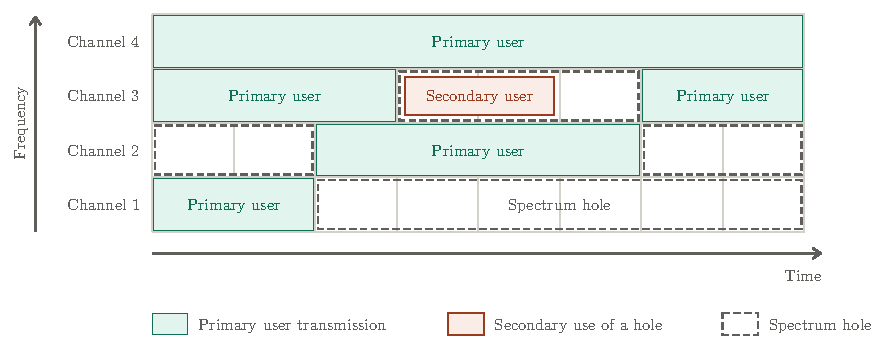
\includegraphics[width=\textwidth]{fig2-spectrum-holes}
  \caption[Spectrum holes in time and frequency]{Spectrum holes in time and frequency at one location (schematic, not to scale). Shaded cells are used by their primary users; an unused cell is a spectrum hole, which a secondary user may occupy until the primary user returns. Drawn after the definition of \textcite[p.~201]{haykin2005}.}
  \label{fig:spectrum-holes}
\end{figure}

Haykin identified three fundamental cognitive tasks: radio-scene analysis, which includes the detection of spectrum holes; channel identification; and transmit-power control with dynamic spectrum management. The first two are carried out in the receiver and the third in the transmitter \parencite[p.~202]{haykin2005}. He also classified the spectrum by measured power into black spaces, occupied by high-power local interferers some of the time; grey spaces, partially occupied by low-power interferers; and white spaces, free of radio frequency interferers except for ambient natural and artificial noise. White spaces, and grey spaces to a lesser extent, are the candidates for secondary use (p.~206).

Spectrum sensing is the function through which a cognitive radio finds these opportunities, and \textcite{yucek2009} described it as one of the most challenging issues in cognitive radio systems (p.~116). The motivation for cognitive radio comes from measurements showing unused resources in frequency, time and space, but cognitive radios must be able to detect very weak primary signals \parencite[pp.~322--323]{axell2010}, because the primary users must be detected in order to avoid causing them harmful interference \parencite{tandra2008}. In Nigeria, \textcite{popoola2018} measured an average occupancy below \pct{10} over \qtyrange{80}{2200}{\mega\hertz} at five sites, and concluded that dynamic spectrum access has a hopeful future in the country (Chapter~1).

This thesis does not build a cognitive radio. It addresses the sensing step on which cognitive radio, and spectrum monitoring generally, depend: deciding whether an LTE carrier is present in an observed slice of spectrum. A band that holds an active LTE carrier offers no opportunity to a secondary user at that place and time; it becomes a spectrum hole only where and when the carrier is absent.

\section{Classical Spectrum Sensing}
\label{sec:sensing}

\subsection{The Detection Problem}
\label{sec:detection-problem}

Spectrum sensing is posed as a binary hypothesis test. Let $y(n)$, $n = 0, \dots, N-1$, be the complex baseband samples observed in one sensing interval. Under the null hypothesis $\mathcal{H}_0$ the band holds noise only; under the alternative $\mathcal{H}_1$ a signal is present \parencite[p.~322]{axell2010}:
\begin{align}
  \mathcal{H}_0 &: \quad y(n) = w(n), \label{eq:h0}\\
  \mathcal{H}_1 &: \quad y(n) = s(n) + w(n), \label{eq:h1}
\end{align}
where $s(n)$ is the signal and $w(n)$ is noise, commonly modelled as independent, zero-mean, circularly symmetric complex Gaussian samples with variance $\sigma^2$ \parencite[p.~322]{axell2010}. A detector computes a test statistic $T$ from the samples and decides $\mathcal{H}_1$ when $T$ exceeds a threshold $\lambda$. Its performance is summarized by two probabilities \parencite[p.~121]{yucek2009}: the probability of detection, $\Pd = \Pr(T > \lambda \mid \mathcal{H}_1)$, and the probability of false alarm, $\Pfa = \Pr(T > \lambda \mid \mathcal{H}_0)$. A high $\Pd$ is wanted, and $\Pfa$ should be kept small so that transmission opportunities are not wasted (p.~121).

The threshold trades $\Pd$ against $\Pfa$. The signal power is difficult to know, since it depends on the transmission and on the distance to the transmitter, so in practice the threshold is chosen to obtain a given false-alarm rate, for which knowledge of the noise variance suffices \parencite[p.~121]{yucek2009}. This is the Neyman--Pearson approach: for a fixed $\Pfa$, the optimal test compares the log-likelihood ratio with a threshold \parencite[p.~322]{axell2010}. The detectors in this thesis are compared in the same way. Each threshold is set on idle validation data for a fixed $\Pfa$ of \pct{1} or \pct{5}, and $\Pd$ is measured at that operating point (Chapter~3).

\subsection{A Taxonomy of Sensing Methods}
\label{sec:taxonomy}

Sensing methods differ mainly in how much they must know about the signal to be detected. \Textcite{yucek2009} reviewed energy detection, waveform-based sensing, cyclostationarity-based sensing, radio identification, matched filtering and other methods such as multitaper and wavelet-based spectral estimation, and compared the main methods by accuracy and complexity (pp.~120--124). Energy detection needs no knowledge of the primary signal, whereas matched filtering needs complete knowledge of it (pp.~120, 123). \Textcite{axell2010} likewise distinguished the energy detector, which assumes no known structure in the signal, from feature detectors that exploit known structure, such as cyclostationarity or the eigenvalue structure of the signal covariance matrix (pp.~322--324). Cooperation among several sensors has been proposed as a remedy for noise uncertainty, fading and shadowing \parencite[p.~124]{yucek2009}; it is outside the scope of this single-receiver study.

\Cref{fig:taxonomy} arranges five non-cooperative methods by the prior knowledge each requires, and \cref{tab:sensing-methods} compares them. Learned detectors, which derive their decision rule from data rather than from a signal model, are shown as a separate branch and are reviewed in \cref{sec:ae,sec:related}. Energy detection, the core baseline of this thesis, is reviewed in the most detail.

\begin{figure}[tbp]
  \centering
  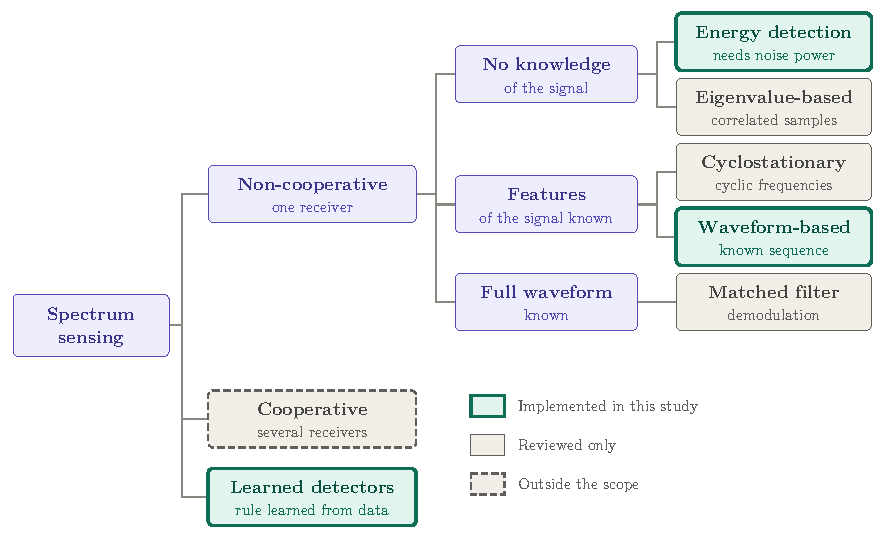
\includegraphics[width=\textwidth]{fig2-sensing-taxonomy}
  \caption[Taxonomy of spectrum sensing methods]{Spectrum sensing methods arranged by the prior knowledge they require. Cooperative sensing is outside the scope of this study; learned detectors are reviewed in \cref{sec:ae,sec:related}. Based on \textcite{yucek2009}, \textcite{axell2010} and \textcite{zeng2009}.}
  \label{fig:taxonomy}
\end{figure}

\begin{table}[tbp]
  \centering
  \small
  \caption[Classical spectrum sensing methods compared]{Classical spectrum sensing methods compared. Sources: \textcite[pp.~120--124]{yucek2009}; \textcite[pp.~322--324]{axell2010}; \textcite{zeng2009}; \textcite{tandra2008}.}
  \label{tab:sensing-methods}
  \begin{tabularx}{\textwidth}{@{} >{\raggedright\arraybackslash}p{2.7cm} >{\raggedright\arraybackslash}X >{\raggedright\arraybackslash}X >{\raggedright\arraybackslash}X @{}}
    \toprule
    Method & Prior knowledge needed & Strengths & Limitations \\
    \midrule
    Energy detection & None about the signal; the noise power, to set the threshold & Simple; low computational and implementation cost; detects any type of signal & Cannot tell primary signals from interference or noise; poor at low signal-to-noise ratio (SNR); SNR wall under noise uncertainty \\
    \addlinespace
    Matched filtering & The complete waveform: bandwidth, frequency, modulation, pulse shaping and frame format; demodulation & Optimal when the signal is known; short sensing time for a given $\Pfa$ & A receiver for every signal type; high complexity and power consumption; SNR wall when channel coherence times are finite \\
    \addlinespace
    Cyclostationary detection & The cyclic frequencies of the signal & Distinguishes noise from modulated signals and different signal types from each other & Worse than energy detection in stationary noise; features can be lost in fading; SNR wall under model uncertainty; sensitive to sampling-clock offsets \\
    \addlinespace
    Eigenvalue-based detection & None about the signal, the channel or the noise power; correlated signal samples & Overcomes noise uncertainty; can beat ideal energy detection for highly correlated signals & A sample covariance matrix and its eigenvalues are needed for every decision \\
    \addlinespace
    Waveform-based detection & A known pattern in the signal: preamble, pilot or synchronization sequence & More reliable and faster to converge than energy detection; improves with pattern length & Applies only to signals with known patterns; susceptible to synchronization errors \\
    \bottomrule
  \end{tabularx}
\end{table}

\subsection{Energy Detection}
\label{sec:ed}

Energy detection is the classical way to detect a signal of unknown form. In the classic analysis by Urkowitz, a deterministic signal of unknown structure is detected in flat, band-limited Gaussian noise of known power spectral density. The received signal is passed through an ideal band-pass filter, its energy over an interval is measured, and the energy is compared with a threshold; the decision statistic then has a noncentral chi-square distribution \parencite[Urkowitz, 1967, as cited in][p.~1606]{kostylev2002}. Received signals often have a random amplitude because of fading, in which case the statistic is no longer chi-square distributed, and \textcite{kostylev2002} derived the detection probability for Rayleigh, Rice, Nakagami and other amplitude distributions (p.~1606). \Cref{fig:ed-block} shows the detector in its sampled form, which is the form used in this thesis.

\begin{figure}[tbp]
  \centering
  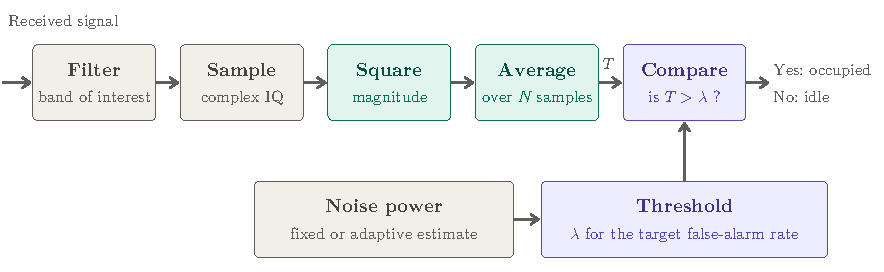
\includegraphics[width=\textwidth]{fig2-energy-detector}
  \caption[Block diagram of the energy detector]{Block diagram of the energy detector in sampled form. The received signal is band-limited and sampled, the squared magnitudes of $N$ samples are averaged, and the average is compared with a threshold $\lambda$ set from the noise power for a target $\Pfa$. Based on \textcite{kostylev2002}, \textcite{axell2010} and \textcite{yucek2009}.}
  \label{fig:ed-block}
\end{figure}

In discrete time, the detector computes the average power of the $N$ samples,
\begin{equation}
  T = \frac{1}{N} \sum_{n=0}^{N-1} \lvert y(n) \rvert^2 ,
  \label{eq:ed-statistic}
\end{equation}
and decides $\mathcal{H}_1$ if $T > \lambda$ \parencite[p.~322]{axell2010}; \textcite{yucek2009} used the same statistic without the factor $1/N$ (p.~121). If the signal is also modelled as zero-mean complex Gaussian, with variance $\sigma_s^2$, the energy detector is the optimal detector in the Neyman--Pearson sense \parencite[p.~322]{axell2010}. The sum $NT$ then follows a scaled chi-square distribution with $2N$ degrees of freedom under both hypotheses, scaled by $\sigma^2/2$ under $\mathcal{H}_0$ and by $(\sigma^2 + \sigma_s^2)/2$ under $\mathcal{H}_1$ \parencite[p.~121]{yucek2009}. Writing $F_{\chi^2_{2N}}$ for the cumulative distribution function of a chi-square variable with $2N$ degrees of freedom, the false-alarm and detection probabilities of \cref{eq:ed-statistic} are
\begin{equation}
  \Pfa = 1 - F_{\chi^2_{2N}}\!\left( \frac{2N\lambda}{\sigma^2} \right), \qquad
  \Pd = 1 - F_{\chi^2_{2N}}\!\left( \frac{2N\lambda}{\sigma^2 + \sigma_s^2} \right),
  \label{eq:ed-pfa-pd}
\end{equation}
and the threshold for a target $\Pfa$ is
\begin{equation}
  \lambda = \frac{\sigma^2}{2N}\, F^{-1}_{\chi^2_{2N}}\!\left(1 - \Pfa\right),
  \label{eq:ed-threshold}
\end{equation}
which follow from the expressions of \textcite[p.~323]{axell2010} for the unnormalized statistic. The SNR is $\gamma = \sigma_s^2/\sigma^2$ \parencite[p.~121]{yucek2009}.

\Cref{eq:ed-threshold} shows the defining property of the method: the threshold depends on the noise variance and not on the signal. Energy detection is universal in the sense that it can detect any type of signal without knowing anything about it, but for the same reason it cannot exploit any knowledge that is available, and it needs the noise power to set its threshold \parencite[p.~323]{axell2010}. \Textcite{yucek2009} described it as the most common way of spectrum sensing because of its low computational and implementation complexity. They listed its main challenges as the selection of the threshold, the inability to tell primary users from interference and noise, and poor performance at low SNR (pp.~120--121). Its performance is also limited when the noise is not stationary or its variance is not known (p.~124).

The noise power is never known exactly. \Textcite{zeng2009} distinguished receiver device noise uncertainty, which arises from the non-linearity of components and from thermal noise that is non-uniform and time-varying, from environmental noise uncertainty, which is caused by other transmissions; because of noise uncertainty, an accurate noise power is very difficult to obtain in practice. A small error in the noise-power estimate causes a significant loss of performance \parencite[p.~121]{yucek2009}. \Textcite{tandra2008} made this precise. They modelled the noise power as known only to lie in an interval $[\sigma_n^2/\rho,\ \rho\,\sigma_n^2]$ around a nominal value $\sigma_n^2$, where $\rho = 10^{\delta/10}$ for an uncertainty of $\delta$ decibels. The energy detector then cannot robustly detect a signal whose power is smaller than the width of that interval, $(\rho - 1/\rho)\,\sigma_n^2$. The result is an \emph{SNR wall},
\begin{equation}
  \mathrm{SNR}_{\mathrm{wall}} = \frac{\rho^2 - 1}{\rho},
  \label{eq:snr-wall}
\end{equation}
below which a detector cannot robustly achieve a useful pair of $\Pfa$ and $\Pd$, however long it observes the channel. An uncertainty of \qty{1}{\decibel}, for example, gives a wall at about \qty{-3.3}{\decibel}, and the number of samples needed grows without bound as the SNR approaches the wall. \Cref{fig:ed-pd-snr} illustrates the effect. Tandra and Sahai further proved that, when the modulation of the signal is unknown, every detector has an SNR wall, and any detector is essentially as non-robust as the energy detector. \Textcite[p.~323]{axell2010} noted that the result was later extended to other model uncertainties, including non-white or non-stationary noise, flat fading, non-ideal filters and finite-precision analogue-to-digital converters, and that noise calibration improves robustness. A related limit comes from the receiver's finite dynamic range. If a radio can quantize voltages only between upper and lower limits, any detector can be rendered useless at low enough SNR, even under moderate noise uncertainty, and all physical radios have such a limit \parencite{tandra2005}. The 8-bit converter of the receiver used here makes this limit concrete (\cref{sec:sdr}).

\begin{figure}[tbp]
  \centering
  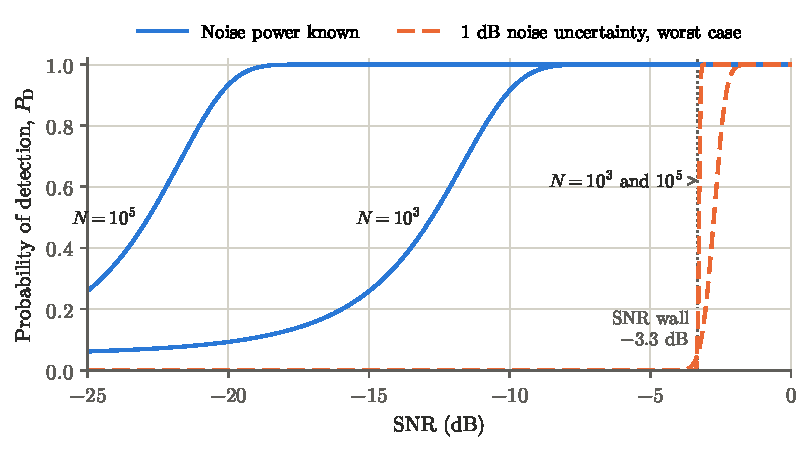
\includegraphics[width=\textwidth]{fig2-ed-pd-snr}
  \caption[Energy detector: detection probability against SNR]{Probability of detection of the energy detector against SNR at $\Pfa = 0.05$, for $N = 10^3$ and $N = 10^5$ complex samples. Solid lines: noise power known exactly, from \cref{eq:ed-pfa-pd,eq:ed-threshold}. Dashed lines: \qty{1}{\decibel} of noise uncertainty, worst case, with the threshold set for the highest noise power in the uncertainty interval and $\Pd$ evaluated at the lowest, following \textcite{tandra2008}. The dotted line marks the SNR wall of \cref{eq:snr-wall}. Analytic curves, not measurements.}
  \label{fig:ed-pd-snr}
\end{figure}

Because its threshold must follow the noise power, a practical energy detector estimates that power. \Textcite{yucek2009} described methods that estimate the noise level dynamically, for example as the smallest eigenvalue of the autocorrelation of the received signal, and then use the estimate to set the threshold for a constant false-alarm rate (CFAR); other methods find the threshold iteratively for a given $\Pfa$ (p.~121). In spectrum occupancy campaigns, measured power levels are compared with pre-established thresholds, which is energy detection in its simplest form \parencite[p.~35]{reyesmoncayo2018}. This thesis uses two variants (Chapter~3). The fixed-threshold detector freezes its noise estimate at calibration. The adaptive detector updates its estimate from recent frames judged idle, and so follows the CFAR principle. Detectors that estimate the noise from neighbouring frequency or time cells, which are often called CFAR detectors, are not implemented (Chapter~1). How the threshold of the energy detector is set also matters when it is used as a baseline for learned detectors, a point taken up in \cref{sec:related-ed}.

\subsection{Matched-Filter Detection}
\label{sec:mf}

If the signal to be detected is perfectly known, the optimal detector is a matched filter \parencite[p.~323]{axell2010}. Its main advantage is the short time it needs to reach a given probability of false alarm or of missed detection \parencite[p.~123]{yucek2009}. It requires, however, that the cognitive radio demodulate the received signal, and hence perfect knowledge of the primary user's signalling features, such as bandwidth, operating frequency, modulation type and order, pulse shaping and frame format. Since a receiver is needed for every signal type, the sensing unit becomes impractically complex, and executing the receiver algorithms consumes much power (p.~123). Coherent detection is not immune to model uncertainty either: with finite channel coherence times it also has an SNR wall, although one that scales more favourably with coherence time than that of cyclostationary detectors \parencite{tandra2008}. Demodulation of LTE is outside the scope of this study (Chapter~1), so the matched filter is not used. Its partial form, correlation with known synchronization sequences, is discussed in \cref{sec:waveform}.

\subsection{Cyclostationary Feature Detection}
\label{sec:cyclo}

Most man-made signals show periodic patterns related to the symbol rate, chip rate, channel code or cyclic prefix. They can be modelled as cyclostationary random processes, whose covariance is periodic in time \parencite[p.~323]{axell2010}. Cyclostationary detectors use the cyclic correlation function of the received signal instead of its power spectral density. Because noise is wide-sense stationary with no correlation while modulated signals are cyclostationary, these detectors can distinguish noise from primary signals, and can also distinguish different types of transmission \parencite[p.~122]{yucek2009}. OFDM signals, used by WiFi, WiMAX, LTE and digital television, have well-known spectral correlation properties, which has made their cyclostationary detection a subject of considerable interest \parencite[p.~323]{axell2010}. The method has costs. Cyclostationary detectors perform worse than energy detectors when the noise is stationary, although they are unaffected by the non-stationary noise caused by co-channel or adjacent-channel interferers, which defeats energy detectors. Their features can be lost through channel fading, model uncertainties cause an SNR wall for them as for energy detectors, and they are vulnerable to sampling-clock offsets \parencite[p.~124]{yucek2009}. They also require the cyclic frequencies of the primary signal \parencite{zeng2009}. They are not implemented in this study.

\subsection{Eigenvalue-Based Detection}
\label{sec:eigen}

Eigenvalue-based detectors exploit the structure of the covariance matrix of the received samples. Under $\mathcal{H}_0$, with white noise, all its eigenvalues equal $\sigma^2$. Under $\mathcal{H}_1$ the eigenvalues of a correlated signal are added to them, so the largest eigenvalues differ markedly from the smallest \parencite[p.~324]{axell2010}. \Textcite{zeng2009} proposed two tests on the sample covariance matrix, the ratio of the maximum to the minimum eigenvalue and the ratio of the average to the minimum eigenvalue, and used random matrix theory to set their thresholds for a given $\Pfa$. Their methods need no knowledge of the signal, the channel or the noise power. They overcome the noise-uncertainty problem and can perform better than an ideal energy detector when the signal samples are highly correlated; energy detection, by contrast, is optimal for independent and identically distributed signals but not for correlated ones. Each decision requires a sample covariance matrix, built from a number of consecutive samples called the smoothing factor, and its extreme eigenvalues. Eigenvalue-based detectors are not implemented in this study.

\subsection{Waveform-Based Detection}
\label{sec:waveform}

Wireless systems often transmit known patterns, such as preambles, midambles, regularly transmitted pilots and spreading sequences, to assist synchronization. Correlating the received signal with a known copy of such a pattern is called waveform-based, or coherent, sensing, and it applies only to systems with known signal patterns \parencite[p.~122]{yucek2009}. \Textcite{yucek2009} reported that it outperforms energy detection in reliability and convergence time, that its performance improves as the known pattern grows longer, and that it needs only short measurements but is susceptible to synchronization errors (p.~122). Because of its coherent processing it is more robust than energy and cyclostationary detection, but it requires a priori knowledge of the primary signal (pp.~123--124).

The LTE PSS and SSS (\cref{sec:lte-sync}) are such patterns. A correlator that searches the observed window for the known synchronization sequences is an instance of waveform-based sensing, and it is included in this study as a baseline (Chapter~3). Because the synchronization signals occupy only the central \qty{1.08}{\mega\hertz} of a carrier, such a correlator can detect a carrier only when the receiver's window covers the carrier's centre (\cref{fig:obs-window}). LTE synchronization signals have also served a different purpose with low-cost receivers: \textcite{calvopalomino2017} used them as a reference for estimating the frequency offset of the local oscillator in RTL-SDR devices (\cref{sec:sdr}).

\section{Software-Defined Radio and the RTL-SDR}
\label{sec:sdr}

A software-defined radio performs in software much of the signal processing that conventional radios perform in dedicated hardware. \Textcite{haykin2005} attributed its practical reality to the convergence of digital radio and computer software, and noted that the term was also coined by Mitola (pp.~202--203). Cognitive radio relies on software-defined radio for reconfigurability (p.~202), and \textcite{mitola1999} regarded software radio as the platform on which cognitive radio would be built (p.~13). For spectrum measurement, the appeal of SDR is that one inexpensive receiver can be retuned and reprogrammed in software for different bands and processing chains.

The RTL-SDR is the cheapest widely used example. RTL-SDR dongles were designed for the reception of digital television (DVB-T), and were found by hardware hackers to be usable as general-purpose SDRs \parencite[p.~1]{rtlsdrblog2024}. \Textcite{calvopalomino2017} attributed their popularity among academics and hobbyists to their very low price (below 25 US dollars), ease of use and the wide availability of open-source SDR software. This study uses the RTL-SDR Blog V4, a version redesigned for SDR use; its specifications are listed in \cref{tab:rtlsdr-v4}. The V4 uses the R828D tuner, whose three inputs are fed by a triplexer that splits the antenna input into high-frequency, very-high-frequency and ultra-high-frequency bands. Simple notch filters for the broadcast AM, FM and digital audio broadcasting (DAB) bands attenuate those signals by a few decibels \parencite[p.~1]{rtlsdrblog2024}.

\begin{table}[tbp]
  \centering
  \caption[Specifications of the RTL-SDR Blog V4]{Specifications of the RTL-SDR Blog V4 relevant to this study. Source: \textcite[p.~1]{rtlsdrblog2024}.}
  \label{tab:rtlsdr-v4}
  \begin{tabularx}{\textwidth}{@{} l >{\raggedright\arraybackslash}X @{}}
    \toprule
    Parameter & Value \\
    \midrule
    Tuner & Rafael Micro R828D \\
    Analogue-to-digital converter & Realtek RTL2832U, 8 bits \\
    Frequency range & \qty{500}{\kilo\hertz} to \qty{1.766}{\giga\hertz} \\
    Bandwidth & \qty{2.56}{\mega\hertz} stable (up to \qty{3.2}{\mega\hertz} with dropped samples) \\
    Input impedance & \qty{50}{\ohm} (typical) \\
    Reference oscillator & Temperature-compensated crystal oscillator (TCXO), \qty{1}{ppm} \\
    Bias tee & \qty{4.5}{\volt}, \qty{180}{\milli\ampere}, switchable in software \\
    Front end & Triplexer with switchable notch filters \\
    Connectors & SMA (antenna); USB-A (host) \\
    Transmit capability & None \\
    \bottomrule
  \end{tabularx}
\end{table}

The internal architecture of the RTL-SDR is not fully documented. \Textcite{calvopalomino2017} therefore modelled it as a generic receiver in which a single local oscillator feeds both the down-conversion stage and the sampling stage, which converts the in-phase and quadrature (IQ) components to digital samples. \Cref{fig:rtlsdr-chain} shows the receive chain used in this study at that functional level. The dongle delivers complex IQ samples over the universal serial bus (USB) to the host, where all further processing takes place in software \parencite{calvopalomino2015}.

\begin{figure}[tbp]
  \centering
  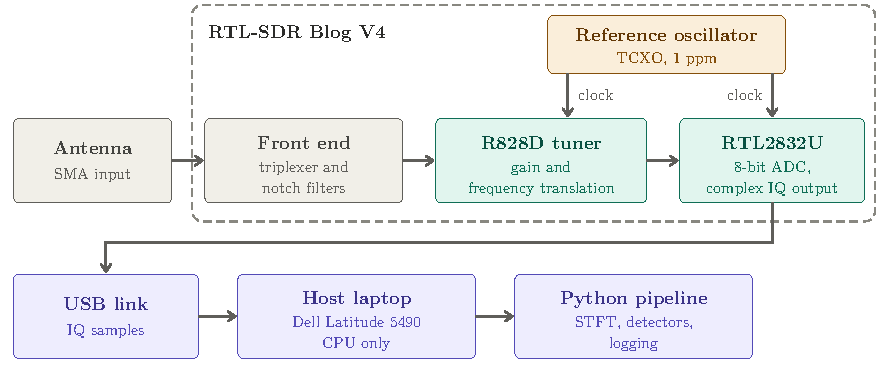
\includegraphics[width=\textwidth]{fig2-rtlsdr-chain}
  \caption[Receive chain of the RTL-SDR and host laptop]{Functional receive chain of the RTL-SDR Blog V4 and the host laptop. The tuner translates the selected band to an intermediate frequency; the RTL2832U digitizes it with an 8-bit converter and delivers complex IQ samples over USB. One reference oscillator clocks both the frequency translation and the sampling. Functional view only: the chips' internal design is not fully documented. Based on \textcite[p.~1]{rtlsdrblog2024} and the receiver model of \textcite{calvopalomino2017}.}
  \label{fig:rtlsdr-chain}
\end{figure}

Low-cost receivers have made continuous and distributed spectrum measurement affordable. \Textcite{calvopalomino2015} demonstrated a sensor platform for large-scale wideband monitoring built from a single-board computer and an RTL-SDR dongle, which scanned the spectrum in steps of \qty{2.4}{\mega\hertz}, the bandwidth sensed at a time with 8-bit resolution. Electrosense extended this approach to a crowdsourced network of low-cost sensors, motivated by how little is known about the actual use of the spectrum over time and space, and made the collected spectrum data available as an open service \parencite{rajendran2018}. Electrosense+ moved the decoding of signals onto the sensors themselves, which used RTL-SDR receivers with temperature-compensated oscillators and sent no raw IQ data to users \parencite{calvopalomino2020}. \Textcite{reyesmoncayo2018} built a low-cost monitor of channel occupancy from an embedded board, Python and an RTL-SDR dongle, noting that the equipment used in earlier occupancy campaigns was too costly for continuous monitoring in many places (p.~34). \Textcite{molinatenorio2021} linked several affordable SDRs, including an RTL-SDR, to sense a wide band in real time with a detector based on wavelets, machine learning and the Higuchi fractal dimension, and reported a \pct{95} probability of success at SNRs above \qty{0}{\decibel} (p.~1). \Textcite{saber2021} used an RTL-SDR to capture real signals for a deep-learning detector (\cref{sec:related-ed}).

Low cost comes with imperfections that a detector must tolerate.
\begin{itemize}
  \item \emph{Frequency offset.} In the dongle used by \textcite{calvopalomino2015}, the oscillator had inaccuracies of the order of \qty{50}{ppm}, which appeared as a temperature-dependent frequency error of a few kilohertz. Using the LTE synchronization signals as a reference, \textcite{calvopalomino2017} found that RTL-SDR models fitted with a temperature-compensated oscillator stayed well within their specified tolerance of \qty{1}{ppm}. The V4 has such an oscillator (\cref{tab:rtlsdr-v4}).
  \item \emph{The direct-current (DC) component.} The processing chain of \textcite{calvopalomino2015} included a DC-removal step before windowing and the fast Fourier transform (FFT).
  \item \emph{Finite dynamic range.} The 8-bit converter limits the range of signal levels that can be represented at once, and a finite dynamic range sets a hard limit on detection at low SNR \parencite{tandra2005}.
  \item \emph{Gain.} The tuner gain is set in software and changes the level of the recorded noise floor, so it is fixed within each capture session and logged (Chapter~3).
\end{itemize}

\section{Time--Frequency Representation}
\label{sec:stft}

An LTE carrier has structure in both time and frequency: its resource blocks occupy contiguous subcarriers, and its synchronization and reference signals recur at fixed intervals (\cref{sec:lte}). The energy statistic of \cref{eq:ed-statistic} discards this structure by summing over the whole observation. A time--frequency representation keeps it, and is the input to the learned detectors in this study.

The short-time Fourier transform (STFT) is the standard such representation. \Textcite{allen1977} defined it as
\begin{equation}
  X_n(e^{j\omega}) = \sum_{m=-\infty}^{\infty} y(m)\, h(n - m)\, e^{-j\omega m},
  \label{eq:stft}
\end{equation}
where the window $h$ selects the portion of the signal $y$ being analysed around time $n$ (p.~1558; their notation adapted). In practice the transform is evaluated at $K$ uniformly spaced frequencies and at frames spaced $R$ samples apart. For complex samples $y(n)$ at a sampling rate $f_s$, frame $\ell$ and frequency bin $k$ give
\begin{equation}
  X(\ell, k) = \sum_{m=0}^{L-1} h(m)\, y(\ell R + m)\, e^{-j 2\pi k m / K}, \qquad k = 0, \dots, K-1,
  \label{eq:stft-discrete}
\end{equation}
with a window of $L$ samples, a bin spacing of $f_s/K$ and a frame spacing of $R/f_s$ seconds. The spectrogram is the squared magnitude, usually in decibels, $S(\ell, k) = 10 \log_{10} \lvert X(\ell, k) \rvert^2$. Arranged over consecutive frames, it forms an image with time along one axis and frequency along the other (\cref{fig:stft}).

\begin{figure}[tbp]
  \centering
  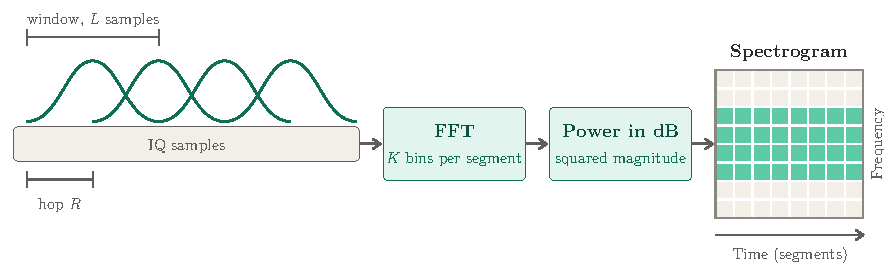
\includegraphics[width=\textwidth]{fig2-stft-spectrogram}
  \caption[From IQ samples to a spectrogram]{From IQ samples to a spectrogram (schematic). Overlapping windowed segments of the IQ stream are transformed with the FFT, and their squared magnitudes in decibels form the columns of a time--frequency image. The shading of the image is illustrative, not data. Based on \textcite{allen1977}.}
  \label{fig:stft}
\end{figure}

Because $X_n$ is the Fourier transform of the product of the signal and the window, it is the convolution of their transforms, so the details of the STFT depend strongly on the window. The window must therefore be chosen to suit the desired time and frequency resolution \parencite[p.~1558]{allen1977}: a long window resolves frequency finely but blurs events in time, and a short window does the reverse (p.~1559). For spectrum displays and signal detection, the STFT serves as a representation of a non-stationary signal and no resynthesis is needed (p.~1559), which is the case in this study.

The shape of the window also matters. A finite record projects any frequency that does not coincide with one of the basis frequencies onto the whole basis set. This spectral leakage results from processing finite-duration records, and windows are weighting functions applied to the data to reduce it \parencite[p.~52]{harris1978}. Windows affect detectability, resolution, dynamic range, confidence and ease of implementation (p.~53). Two of Harris's figures of merit bear directly on detection. The equivalent noise bandwidth of a window is the width of the rectangular filter that has the same peak power gain and accumulates the same noise power; a larger equivalent noise bandwidth admits more noise into each bin and reduces the processing gain (pp.~54, 56). The peak sidelobe level and the rate at which sidelobes fall off indicate how well a window suppresses leakage from strong signals into distant bins (p.~57). For an occupancy detector, leakage from a strong carrier can raise bins outside it, while the equivalent noise bandwidth sets the noise level in each bin, so the window affects both the idle and the occupied statistics.

Spectrograms and averaged power spectra are the usual inputs to learned spectrum detectors. \Textcite[p.~4]{xu2021} and \textcite[p.~4]{tian2022} computed STFT spectrograms of captured IQ data and down-sampled them to $64 \times 64$ images. \Textcite{tandiya2018} used spectrogram images from a waterfall display, and \textcite{rajendran2020} used patches of consecutive power spectral density (PSD) vectors. In this study the spectrogram, or a frame of it, is the input to the autoencoders and to the linear reconstruction baseline of \cref{sec:ae-pca} (Chapter~3).

\section{Autoencoders and Anomaly Detection}
\label{sec:ae}

The autoencoders studied in this thesis are its AI-based detectors. They are neural networks \parencite[p.~499]{goodfellow2016} and therefore belong to machine learning, which is used for many, though not all, approaches to AI \parencite[p.~9]{goodfellow2016}. This section describes how they detect anomalies, how they relate to PCA, the architectures compared, the variational autoencoder, and how their thresholds are set.

\subsection{Anomaly Detection with Normal-Only Training}
\label{sec:ae-anomaly}

An anomaly is an observation that deviates considerably from some concept of normality \parencite{ruff2021}. In the unsupervised setting, a model is trained on unlabelled data that are assumed to be drawn from the normal distribution; such training data are called clean, although in practice they may contain noise or contamination \parencite{ruff2021}. Reconstruction-based methods learn a model that reconstructs normal data well, and they detect anomalies by their failure to reconstruct them accurately; they are among the earliest and most common neural approaches to anomaly detection \parencite{ruff2021}.

Most spectrum anomaly detectors treat a band with its usual signals as normal and an unexpected signal as the anomaly (\cref{sec:related-anomaly}). This study inverts that arrangement. Idle spectrum, the receiver noise and whatever the environment contributes in a band without an LTE carrier, is the normal class, and an LTE carrier is the anomaly to be detected. \Textcite{torio2025} framed transmission detection in the same way, assuming that the normal state of a channel is the absence of transmissions (p.~5). A practical consequence is the need for clean idle training data: any LTE energy left in the training frames would be learned as normal, which is why the idle window is surveyed and checked before any idle data are captured (\cref{sec:m-survey}).

\subsection{Principal Component Analysis and the Autoencoder}
\label{sec:ae-pca}

Principal component analysis (PCA) finds an orthogonal basis that maximizes the variance of the centred data. Its components are the eigenvectors of the empirical covariance matrix with the largest eigenvalues. Equivalently, PCA finds the projection onto a $d$-dimensional linear subspace that minimizes the mean squared reconstruction error, and in that form it can be regarded as the default reconstruction baseline for anomaly detection \parencite{ruff2021}. With the $d$ leading eigenvectors as the rows of a $d \times D$ matrix $\mathbf{W}$, the reconstruction error of an input $\mathbf{x}$ is $\lVert \mathbf{x} - \mathbf{W}^{\top}\mathbf{W}\mathbf{x} \rVert^2$.

An autoencoder is a neural network trained to copy its input to its output. It consists of an encoder $\mathbf{h} = f(\mathbf{x})$, which produces a code, and a decoder $\mathbf{r} = g(\mathbf{h})$, which produces a reconstruction, and it is trained to minimize a loss that penalizes the difference between $g(f(\mathbf{x}))$ and $\mathbf{x}$, such as the mean squared error \parencite[pp.~499--500]{goodfellow2016}. When the code has fewer dimensions than the input, the autoencoder is called undercomplete, and it is forced to capture the most salient features of the training data (p.~500). For $n$ training inputs $\mathbf{x}_i$, each with $D$ elements, the training objective is
\begin{equation}
  \min_{f,\, g} \; \frac{1}{n} \sum_{i=1}^{n} \bigl\lVert \mathbf{x}_i - g\bigl(f(\mathbf{x}_i)\bigr) \bigr\rVert^2 ,
  \label{eq:ae-objective}
\end{equation}
and the anomaly score of a new input is its reconstruction error, $e(\mathbf{x}) = \frac{1}{D} \lVert \mathbf{x} - g(f(\mathbf{x})) \rVert^2$, the mean squared error (MSE) over its $D$ elements \parencite{ruff2021}. With a linear decoder and the mean squared error as loss, an undercomplete autoencoder learns the same subspace as PCA; with non-linear encoder and decoder functions it can learn a more powerful, non-linear generalization of PCA \parencite[p.~500]{goodfellow2016}. \Textcite{ruff2021} likewise noted that a linear autoencoder with a bottleneck recovers the subspace spanned by the PCA eigenvectors. PCA is therefore the natural baseline for an autoencoder: if the non-linear model does not detect better than PCA, its extra complexity is not justified. That comparison is part of RQ2.

\subsection{Fully Connected versus Convolutional Architectures}
\label{sec:ae-architectures}

A spectrogram can be fed to an autoencoder in two ways. A fully connected autoencoder flattens it into a vector and uses dense layers, in which every output unit interacts with every input unit through its own parameter. A convolutional autoencoder keeps the two-dimensional layout and uses convolutional layers. \Textcite{goodfellow2016} identified three properties of convolution that help a learning system (pp.~329--334). The first is sparse interactions: the kernel is smaller than the input, so a layer with $m$ inputs and $n$ outputs needs only $k \times n$ parameters for a kernel of $k$ elements instead of $m \times n$. The second is parameter sharing: the same kernel is applied at every position. The third, which follows from parameter sharing, is equivariance to translation: when a pattern in the input shifts, its representation shifts in the same way. \Textcite{masci2011} made the same point for autoencoders. Fully connected autoencoders ignore the two-dimensional structure of an image, which causes problems with realistically sized inputs and introduces redundancy in the parameters, forcing every feature to span the entire input. Convolutional autoencoders share their weights among all locations in the input and so preserve spatial locality (p.~54).

A worked example shows the scale of the difference. A $64 \times 64$ spectrogram, the size used by \textcite{xu2021} and \textcite{tian2022}, has $D = 4096$ elements. A dense layer of 256 units applied to the flattened spectrogram needs $4096 \times 256 + 256 = \num{1048832}$ parameters. A convolutional layer with 32 kernels of $3 \times 3$ elements needs $32 \times 9 + 32 = 320$, whatever the size of the input (\cref{fig:ae-architectures}).

\begin{figure}[tbp]
  \centering
  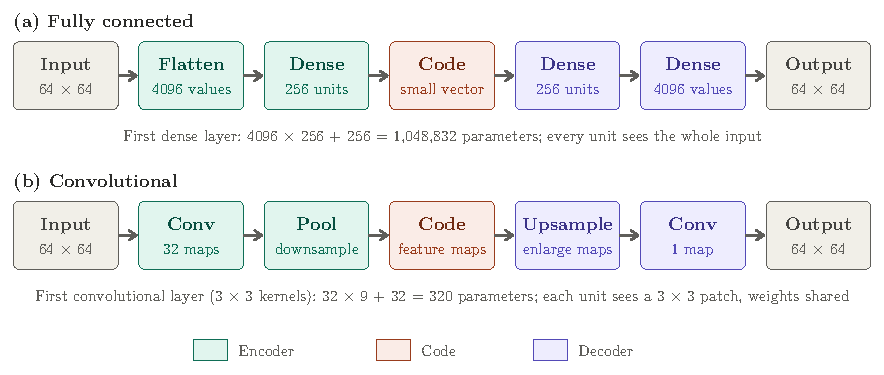
\includegraphics[width=\textwidth]{fig2-ae-architectures}
  \caption[Fully connected and convolutional autoencoders]{Fully connected (top) and convolutional (bottom) autoencoders for a $64 \times 64$ spectrogram. The dense encoder connects every input element to every unit; the convolutional encoder applies the same small kernels at every position. Parameter counts are for the first encoder layer. The layer sizes are illustrative; the architectures used in this study are given in Chapter~3. Based on \textcite[pp.~329--334]{goodfellow2016} and \textcite[p.~54]{masci2011}.}
  \label{fig:ae-architectures}
\end{figure}

These properties suit the spectrogram of an LTE carrier. The carrier appears as a band of raised power over contiguous frequency bins that persists in time, and where it falls within the window depends on the tuning (\cref{fig:obs-window}). A convolutional layer can detect the same local pattern, such as the edge of a carrier, wherever it occurs, whereas a dense layer must learn it separately at every position. This is the argument for the convolutional autoencoder as the primary model in this study. It is an argument, not a result. The empirical evidence on the two architectures is mixed. With the percentile score of \textcite{tian2022}, a fully connected variational autoencoder achieved a higher area under the curve than a convolutional one for Gaussian minimum-shift keying (GMSK) and chirp anomalies and a lower one for quadrature phase-shift keying (QPSK) and 16-point quadrature amplitude modulation (16QAM) anomalies (p.~8). \Textcite{xu2021} found the convolutional variant better by 0.016 in area under the curve, and better at low false-positive rates (p.~5). \Textcite{baset2023} found a shallow convolutional autoencoder sufficient for aviation signals; adding layers increased the prediction time without significantly improving detection. The architectural choice is therefore tested directly in this study, with a fully connected autoencoder trained on the same data (Chapter~4).

\subsection{Variational Autoencoders and Percentile Scores}
\label{sec:ae-vae}

A variational autoencoder (VAE) is a probabilistic version of the autoencoder. \Textcite{kingma2014} introduced a recognition model $q_{\phi}(\mathbf{z} \mid \mathbf{x})$, which approximates the intractable posterior distribution of a latent code $\mathbf{z}$ and acts as a probabilistic encoder, and a generative model $p_{\theta}(\mathbf{x} \mid \mathbf{z})$, which acts as a probabilistic decoder. Both are trained jointly by maximizing a lower bound on the likelihood of the data, which a reparameterization makes amenable to standard stochastic gradient methods; when the recognition model is a neural network, the result is the variational autoencoder (pp.~1--3).

For spectrum anomaly detection, \textcite{tian2022} trained VAEs on spectrograms of normal data and argued that the mean squared error pays equal attention to every part of the spectrum, which dilutes the effect of anomalies that are short or narrow in frequency (p.~2). They proposed a percentile (PER) score, which combines high percentiles of the pixel-level reconstruction errors in the background and signal regions of the spectrogram (p.~4). For QPSK anomalies, it raised the recall from \pct{80} to \pct{93} at a false-alarm rate of \pct{5} (p.~6). \Textcite{xu2021} proposed a related score that weights the reconstruction error towards low-amplitude, noise-like regions of the spectrogram, to which an anomaly raises the noise floor of the reconstruction (pp.~1, 3). Both scores show that how the reconstruction error is summarized can matter as much as the model. This study includes a VAE with the percentile score as a comparison with the MSE score (Chapter~3).

\subsection{Setting the Threshold}
\label{sec:ae-threshold}

An anomaly score becomes a detector only when a threshold is applied to it. A threshold can always be derived from the empirical distribution of the anomaly scores \parencite{ruff2021}. Studies differ in which scores they use and how. \Textcite{rajendran2019} applied an $n$-sigma rule to the reconstruction and discriminator losses, using their mean and standard deviation on the training data, with $n$ chosen empirically. \Textcite{baset2023} set the threshold at the 98th percentile of the reconstruction errors on the training data, which corresponds to a false-positive rate of \pct{2} on those data. \Textcite{torio2025} set it a chosen number of decibels above the activity of the least active channel, which they took as a noise-only reference (p.~9). For supervised detectors, \textcite{gao2019} noted that the lack of precise control of the false-alarm rate is a drawback of deep-learning detectors.

In this study every detector, learned or classical, is thresholded in the same way. The threshold is the empirical $(1 - \Pfa)$ quantile of the detector's scores on idle validation frames, which are held out from training, for a target $\Pfa$ of \pct{1} or \pct{5} (\cref{fig:threshold}; Chapter~3). This is the empirical counterpart of the Neyman--Pearson threshold of the energy detector (\cref{sec:detection-problem}). Because the validation frames are not used for training, the false-alarm rate they fix is not biased by any fitting of the model to its own training data, and all detectors are compared at the same operating points.

\begin{figure}[tbp]
  \centering
  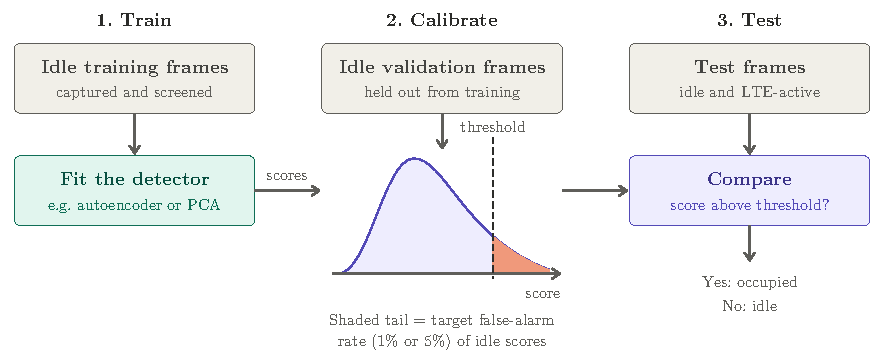
\includegraphics[width=\textwidth]{fig2-threshold-calibration}
  \caption[Threshold calibration on idle validation data]{Detection by reconstruction error with a threshold calibrated on idle data. The model is trained on idle frames only; its scores on held-out idle validation frames set the threshold at the $(1 - \Pfa)$ quantile; test frames whose score exceeds the threshold are declared occupied. The distribution sketch is schematic, not data. The same calibration is applied to every detector in this study.}
  \label{fig:threshold}
\end{figure}

\section{Related Work}
\label{sec:related}

This section reviews the studies closest to this thesis in two strands: learned spectrum anomaly detection (\cref{sec:related-anomaly}) and learned spectrum sensing compared with energy detection (\cref{sec:related-ed}). Low-cost monitoring systems were reviewed in \cref{sec:sdr}. \Cref{sec:related-practice} compares how the studies were evaluated, and \cref{tab:related-anomaly,tab:related-sensing} summarize them.

\subsection{Learned Spectrum Anomaly Detection}
\label{sec:related-anomaly}

Early work used prediction rather than reconstruction. \Textcite{oshea2016} trained recurrent predictors, chiefly a two-layer long short-term memory (LSTM) network, on raw IQ recordings made over the air with a USRP B200-mini in FM broadcast, cellular (GSM and LTE) and industrial, scientific and medical (ISM) bands (pp.~2--3). They injected five classes of synthetic anomalies into the recordings and detected them from the likelihood of the prediction error (pp.~2, 4). The neural predictors slightly outperformed a Kalman-filter predictor, with slightly larger improvements in the cellular bands, whose carriers have a more regular temporal structure (p.~6). \Textcite{tandiya2018} trained a deep predictive coding network on sequences of spectrogram images and spectral correlation images of normal network behaviour, generated in GNU Radio Companion, and reported detection of nearly \pct{100} at high SNR and \pct{90} at medium SNR for a false-alarm rate of 0.15 with the spectral correlation images.

Reconstruction models followed. \Textcite{rajendran2019} proposed SAIFE, an adversarial autoencoder that detects anomalies in PSD data and learns interpretable features in a semi-supervised way. They evaluated it on synthetic data, on sweeps recorded with a HackRF receiver in two Belgian cities and on data from Electrosense sensors, with synthetic anomalies injected into the real captures and the data split at random into equal training and test sets. \Textcite{rajendran2020} adapted SAIFE to crowdsourced sensing, using 56 days of spectrogram data from four Electrosense sensors built on low-cost RTL-SDR receivers sampling at \qty{2.4}{MS/s}. They trained on seven days and tested on the other 49, taken from non-adjacent periods. At constant false-alarm rates of \pct{5} and \pct{10}, SAIFE detected injected anomalies better than a one-class support vector machine, an isolation forest and the lightweight on-line detector of anomalies (LODA). The authors also observed that unsupervised threshold selection is difficult even with full knowledge of the anomalies.

Variational autoencoders on spectrograms were studied in the ISM band at \qty{2.4}{\giga\hertz}. \Textcite{xu2021} used a single capture of about \qty{41}{\minute}, split at random into training and test spectrograms, with chirp anomalies added digitally (p.~4). \Textcite{tian2022} recorded normal data in a laboratory and created anomalies by transmitting QPSK, 16QAM, GMSK and chirp signals from a second USRP, again with a random split of the normal data (p.~4). Neither study compared its detector with energy detection; Tian et al.\ compared their percentile score with MSE and mean absolute error scores and with classical outlier detectors (p.~6).

\Textcite{baset2023} built AviSense, a real-time monitor of aviation bands that combines a signal detector with autoencoder-based anomaly classification. Its signal detector is an energy detector refined by a spectral flatness measure, with a threshold recomputed at run time from blocks judged to be noise. When a threshold computed on one day was applied on another day, \pct{74.20} of the noise blocks were passed as signal, against \pct{32.79} to \pct{49.54} on the day of computation, which led the authors to conclude that a static threshold is impractical. Detected signals were then classified as normal or anomalous by shallow convolutional autoencoders trained on normal data only. Normal data were recorded at four locations with a USRP X310, a HackRF One or an RTL-SDR, and the test data deliberately varied the receiver, its gain, and the day, location and time of collection. AviSense ran on the central processing unit (CPU) of a laptop, and it is the only study in this group to report inference throughput.

\Textcite{torio2025} came closest to the present design. Treating the absence of transmissions as the normal state, they trained a one-dimensional convolutional autoencoder on synthetic Rayleigh-distributed noise sequences and applied it to day-long amplitude recordings from a regulator's monitoring station in the very high frequency (VHF) maritime and land mobile bands (pp.~4--5, 7). They compared it with a detector based on channel power, whose threshold was also set relative to the least active channel (p.~8). The two methods detected practically the same intervals. The autoencoder was more sensitive to low-power transmissions, whereas the power detector tolerated calibration imperfections better and needed no graphics processor (pp.~12, 14). They reported no probabilities of detection or false alarm.

\subsection{Learned Sensing versus Energy Detection}
\label{sec:related-ed}

A second strand trains supervised classifiers on labelled signal and noise examples and compares them with classical detectors. \Textcite{gao2019} trained DetectNet, a network of convolutional and LSTM layers, on single-carrier signals generated in simulation following the conventions of the RadioML2016.10a dataset. At a $\Pfa$ of \pct{5.92} and a $\Pd$ of \pct{90}, its SNR wall was \qty{3.15}{\decibel} lower than that of the energy detector for 16QAM signals, and for GFSK it was about \qty{5}{\decibel} lower across sample lengths. The energy detector's SNR wall, however, was calculated from a formula rather than measured on the same simulated frames. \Textcite{zheng2020} trained a residual convolutional network on power spectra and reported better detection than maximum--minimum eigenvalue and entropy detectors at false-alarm probabilities of 0.1, 0.01 and 0.001, particularly at low SNR. Their training data were simulated, and in their one over-the-air test the captured signals of the Aircraft Communications Addressing and Reporting System (ACARS) were combined with simulated noise. \Textcite{peng2020} trained a convolutional network on simulated raw IQ samples. It outperformed an energy detector and approached the optimal detector when tested on data like its training data, but its performance degraded significantly when the signal or channel changed, and unsupervised domain adaptation still left it worse than the energy detector. Fine-tuning with a few hundred labelled examples from the new domain restored its advantage.

Two studies point the other way or qualify the comparison. \Textcite{grosu2021}, using simulated OFDM signals over additive white Gaussian noise (AWGN), flat-fading and frequency-selective channels, found that an energy detector with a threshold set adaptively from the noise variance and a target false-alarm rate outperformed their neural network on average, especially at low SNR. A network trained on data concentrated in a narrow SNR range outperformed the energy detector only within that range (p.~11). \Textcite{saber2021} captured amplitude- and frequency-shift-keyed signals at \qty{433}{\mega\hertz} with an RTL-SDR and reported a $\Pd$ of 0.994 for their deep-learning classifier against 0.961 for energy detection. The detectors were compared at different false-alarm probabilities, however (0.0023 and 0.0120), the energy detector's threshold rule is described only by reference to earlier work, and the classifier they call a convolutional network is described in the text as fully connected. \Textcite{zeghdoud2023}, as reported in their abstract, found a detector that combines a convolutional neural network (CNN) with an LSTM network better than CNN, LSTM and energy detectors at low SNR in numerical simulation, and implemented real-time sensing on a USRP.

\subsection{Evaluation Practice}
\label{sec:related-practice}

\Cref{tab:related-anomaly,tab:related-sensing} show how differently these studies were evaluated, and the differences limit what can be concluded from them.

\begin{itemize}
  \item \emph{Data.} Five studies used simulated data only \parencite{tandiya2018,gao2019,zheng2020,peng2020,grosu2021}. Most studies with real captures injected synthetic anomalies into them \parencite{oshea2016,rajendran2019,rajendran2020,xu2021}; only \textcite{tian2022} and \textcite{baset2023} transmitted their anomalies over the air. No study evaluated the occupancy of an LTE downlink band; LTE appears only as one of the recorded bands of \textcite{oshea2016}.
  \item \emph{What is normal.} The anomaly detectors treat a band with its usual signals as normal. Only \textcite{torio2025} treated the absence of transmissions as normal, and their model was trained on synthetic noise. None of the studies trained a detector on captured idle spectrum.
  \item \emph{Energy-detector baselines.} Most anomaly-detection studies included no energy detector. Where one was included, its threshold was set adaptively from the noise variance \parencite{grosu2021}, relative to a reference channel \parencite{torio2025}, from an analytical formula \parencite{gao2019}, or in a way that is not described \parencite{saber2021,peng2020}. The finding of \textcite{baset2023} that a static energy threshold fails from one day to the next shows why the choice matters.
  \item \emph{Operating points.} Several studies reported results at fixed false-alarm rates \parencite{rajendran2020,tian2022,zheng2020,peng2020,gao2019,grosu2021}; others reported only receiver operating characteristic (ROC) curves, the area under them (AUC), or accuracy. Where thresholds were derived from data, they came from training-data statistics \parencite{rajendran2019,rajendran2020,baset2023}. None of the studies described calibrating a threshold on a separate held-out set of noise-only data.
  \item \emph{Splits and variability.} Random splits were common \parencite{rajendran2019,xu2021,tian2022}. Only \textcite{rajendran2020} separated training and test data by time, and \textcite{baset2023} varied receiver, gain, day and location in their test data. None of the thirteen studies reported confidence intervals.
  \item \emph{Computation.} Training on graphics processors was common \parencite{tandiya2018,rajendran2020,zheng2020}, and the autoencoder of \textcite{torio2025} required one. Only \textcite{baset2023} reported inference throughput on a laptop CPU, and none reported per-frame latency.
\end{itemize}

\begin{table}[tbp]
  \centering
  \footnotesize
  \setlength{\tabcolsep}{3pt}
  \caption[Related studies: learned spectrum anomaly detection]{Related studies of learned spectrum anomaly detection. ED: energy detector; FAR: false-alarm rate; ROC: receiver operating characteristic. The last row describes the design of this study, not its results.}
  \label{tab:related-anomaly}
  \begin{tabularx}{\textwidth}{@{} >{\raggedright\arraybackslash}p{2.1cm} >{\raggedright\arraybackslash}X >{\raggedright\arraybackslash}X >{\raggedright\arraybackslash}p{2.0cm} >{\raggedright\arraybackslash}p{1.9cm} >{\raggedright\arraybackslash}p{1.9cm} @{}}
    \toprule
    Study & Data and receiver & Task and model & ED baseline & Fixed FAR & Split \\
    \midrule
    \textcite{oshea2016} & Real recordings incl.\ GSM and LTE bands, USRP B200-mini; synthetic anomalies & Anomaly; LSTM predictor, normal-only & None (Kalman predictor) & Constant FAR, value not stated & Not stated \\
    \textcite{tandiya2018} & Simulated in GNU Radio & Anomaly; predictive coding on spectrogram and correlation images, normal-only & None & One point, 0.15 & Not stated \\
    \textcite{rajendran2019} & Synthetic; real HackRF and Electrosense PSD; injected anomalies & Anomaly; adversarial autoencoder & None & None (ROC) & Random \\
    \textcite{rajendran2020} & Real Electrosense RTL-SDR PSD, 56 days; injected anomalies & Anomaly; adversarial autoencoder, active learning & None & \pct{5}, \pct{10} & By time (7 / 49 days) \\
    \textcite{xu2021} & Real USRP capture, ISM band, one session; added chirps & Anomaly; convolutional and dense VAE & None & None (ROC) & Random \\
    \textcite{tian2022} & Real USRP laboratory capture, ISM band; transmitted anomalies & Anomaly; convolutional and dense VAE, percentile score & None & Recall at \pct{5} & Random \\
    \textcite{baset2023} & Real aviation bands, USRP X310, HackRF One, RTL-SDR; chamber and RadioML anomalies & Anomaly; shallow convolutional autoencoders & Front-end stage with adaptive threshold & Training-error percentile (\pct{2}) & Test varies receiver, gain, day, place \\
    \textcite{torio2025} & Real VHF amplitude recordings; training on synthetic noise & Transmission detection; 1-D convolutional autoencoder & Power detector, relative threshold & None & None (synthetic training) \\
    \addlinespace
    This study & Real LTE downlink captures, RTL-SDR Blog V4; captured idle data & Occupancy; convolutional and dense autoencoders, VAE, PCA, normal-only & Fixed and adaptive, same frames & \pct{1}, \pct{5} & By capture session \\
    \bottomrule
  \end{tabularx}
\end{table}

\begin{table}[tbp]
  \centering
  \footnotesize
  \setlength{\tabcolsep}{3pt}
  \caption[Related studies: learned spectrum sensing]{Related studies of learned spectrum sensing compared with classical detectors. ED: energy detector; FAR: false-alarm rate. Zeghdoud et al.\ (2023) is summarized from its abstract only. The last row describes the design of this study, not its results.}
  \label{tab:related-sensing}
  \begin{tabularx}{\textwidth}{@{} >{\raggedright\arraybackslash}p{2.1cm} >{\raggedright\arraybackslash}X >{\raggedright\arraybackslash}X >{\raggedright\arraybackslash}p{2.0cm} >{\raggedright\arraybackslash}p{1.9cm} >{\raggedright\arraybackslash}p{1.9cm} @{}}
    \toprule
    Study & Data and receiver & Task and model & ED baseline & Fixed FAR & Split \\
    \midrule
    \textcite{gao2019} & Simulated single-carrier signals & Sensing; supervised CNN--LSTM & Analytical SNR wall & \pct{5.92}; \pct{7} to \pct{9} & 3:1:1, method not stated \\
    \textcite{zheng2020} & Simulated; ACARS signals with simulated noise & Sensing; supervised residual CNN & None (eigenvalue, entropy) & 0.1, 0.01, 0.001 & Separate simulated sets \\
    \textcite{peng2020} & Simulated & Sensing; supervised CNN on IQ & Yes, threshold not described & 0.1 & Separate simulated sets \\
    \textcite{grosu2021} & Simulated OFDM & Sensing; supervised convolutional--LSTM & Adaptive threshold & 0.01 & Separate simulated sets \\
    \textcite{saber2021} & Real RTL-SDR laboratory captures, \qty{433}{\mega\hertz} & Sensing; supervised network & Yes, threshold not described & None (unequal FAR) & Not stated \\
    \textcite{zeghdoud2023} & Simulation; USRP demonstration & Sensing; supervised CNN--LSTM & Yes, in simulation & Not known & Not known \\
    \addlinespace
    This study & Real LTE downlink captures, RTL-SDR Blog V4; captured idle data & Occupancy; convolutional and dense autoencoders, VAE, PCA, normal-only & Fixed and adaptive, same frames & \pct{1}, \pct{5} & By capture session \\
    \bottomrule
  \end{tabularx}
\end{table}

\section{Research Gap}
\label{sec:gap}

Each element of the present design has precedents. Real captures from low-cost RTL-SDR receivers have been used for learned detection \parencite{rajendran2020,saber2021,baset2023}. Treating the absence of transmissions as the normal state has been tried \parencite{torio2025}, as has separating training and test data by time \parencite{rajendran2020}. Results have been reported at fixed false-alarm rates \parencite{zheng2020,grosu2021}, adaptive energy-detector thresholds have been used \parencite{grosu2021,baset2023}, and throughput on a laptop CPU has been measured \parencite{baset2023}. No reviewed study combines these elements, and none addresses the occupancy of an LTE downlink band.

The combination matters because the elements interact. The comparison between learned detectors and energy detection is mixed, and most of the evidence comes from simulation, from energy detectors whose thresholds were not tuned on the same data, or from comparisons at unequal false-alarm rates (\cref{sec:related-ed}). The one study that trained an autoencoder on noise used synthetic noise, measured no detection or false-alarm probabilities, and analysed one day of recordings \parencite{torio2025}. The one result on threshold stability across days concerns a static energy threshold \parencite{baset2023}; no study has asked whether a learned detector holds its calibrated false-alarm rate when the noise floor changes between sessions, although its input normalization and threshold are fixed once trained.

The gap is therefore the following. No study has evaluated, on real LTE downlink captures from a low-cost RTL-SDR, an autoencoder trained only on captured idle spectrum against carefully tuned classical baselines, including fixed-threshold and adaptive-threshold energy detectors, a PCA detector and a \syncsignal{} correlator. Such an evaluation must compare all detectors on identical frames, at false-alarm rates calibrated on held-out idle data, across capture sessions, with uncertainty estimates and with the computational cost of each detector measured on the hardware that would run it. The research questions of Chapter~1 address these points: RQ1 the comparison with energy detection at fixed $\Pfa$, RQ2 the value of non-linearity over PCA and the other baselines, RQ3 generalization across sessions and gain settings, RQ4 latency and throughput on the laptop's CPU, and RQ5 the effect of architecture and score.

\section{Summary}
\label{sec:lit-summary}

This chapter reviewed the background and related work for the study. An active LTE downlink carrier transmits reference signals in every subframe and synchronization signals every \qty{5}{\milli\second}, the latter only in its central \qty{1.08}{\mega\hertz}, while the RTL-SDR observes at most about \qty{2.56}{\mega\hertz} at a time. Occupancy detection is the sensing function on which cognitive radio and spectrum monitoring depend. Of the classical sensing methods, energy detection needs no knowledge of the signal, but its threshold depends on the noise power, and uncertainty in that power produces an SNR wall. Waveform-based detection with the LTE synchronization signals is more reliable but works only when the window covers the centre of the carrier. Low-cost SDRs make continuous monitoring affordable, at the price of hardware imperfections. Spectrograms preserve the time--frequency structure that energy detection discards. Autoencoders, linear PCA and variational autoencoders detect anomalies by reconstruction error, and convolutional architectures exploit the local, shift-invariant structure of spectrograms, although the evidence for them over dense models is mixed. The related work leaves open whether an autoencoder trained on captured idle spectrum outperforms tuned classical detectors on real LTE captures at fixed false-alarm rates and across sessions. Chapter~3 describes the method used to answer that question.
